\chapter{Выпуклые структуры в экономике}





{\conts{Выпуклые множества и вогнутые функции.
--- Теоремы отделимости. --- Лемма Минковского-Фаркаша. ---
Эффективные точки на выпуклых множествах. --- Оптимальность по
Парето. --- Общая теорема Куна-Таккера. --- Теорема Куна-Таккера для
дифференцируемых функций.}}


\section{Выпуклые множества и вогнутые функции\protect\footnote{\cite{Gale:1963},
\cite{Takayama:1985}, \cite{Braverman:1976}.}}

В данном разделе мы введем понятия \emph{отрезка}, \emph{выпуклой
комбинации}, \emph{выпуклого множества}, \emph{вогнутой функции}. В
рамках раздела мы трактуем вектор и точку множества, как синонимы
(см. также раздел~\vref{app:vectors} математического приложения).

\subsection{Выпуклые множества}

Введем ряд геометрических понятий в $n$-мерном пространстве $\R^n$,
являющихся непосредственным обобщением соответствующих понятий в
двух- и трехмерном пространствах.

Если в двумерном пространстве заданы два вектора (точки) $\vc{x}'$ и
$\vc{x}''\!$, то вектор $(\vc{x}'' - \vc{x}')$ есть вектор,
направленный из точки $\vc{x}'$ в точку $\vc{x}''$ (см. Рис.~
\ref{fig:segment}).



Поэтому вектор $\vc{x}^\theta = \theta \,
\vc{x}'+(1-\theta)\,\vc{x}''$ при некотором $\theta$, большем нуля и
меньшем единицы, лежит на \emph{отрезке}, соединяющем точки
$\vc{x}'$ и $\vc{x}''\!$. Меняя $\theta$ от нуля до единицы, мы
получаем все точки этого отрезка. Аналогично, понятие отрезка можно
ввести и в $n$-мерном пространстве.

\input{pics/segment.TpX}

\begin{dfn}

Пусть заданы две точки $\vc{x}'$ и $\vc{x}''\!$, лежащие в множестве
$\st{X} \subset \R^n$. \dw{Отрезком}\index{отрезок} называется
множество, каждая точка $\vc{x}^\theta$ которого удовлетворяет
соотношению $\vc{x}^\theta = \theta \, \vc{x}' +
(1-\theta)\,\vc{x}''$ для любого $0 \leq \theta \leq 1$. \end{dfn}

Точку $\vc{x}^\theta$ в этом случае называют \emph{выпуклой
комбинацией} точек $\vc{x}'$ и $\vc{x}'\!$. В общем случае можно
привести следующее определение выпуклой комбинации точек.

\begin{dfn}

Пусть заданы $m$ точек $\vc{x}^1, \vc{x}^2, \ldots, \vc{x}^m$
множества ${\st{X} \in \R^n}$. Точка $\vc{x}^\theta$ называется их
\dw{выпуклой комбинацией}\index{выпуклая комбинация}, если

\[
\vc{x}^\theta = \sum \limits_{j=1}^{m} \theta_j \vc{x}^j,
\]

\noindent где $0 \leq \theta_j \leq 1$, $\theta_j \in \R$, $j=1
\ldots m$, и $\sum \limits _{j=1}^{m} \theta_j=1$. \end{dfn}

С учетом приведенных выше определений представляется полезным ввести
еще два понятия: понятие \emph{прямой} и \emph{луча}.

\begin{dfn}(\cite{Kapustin:2001})

Пусть заданы точки $\vc{x}', \vc{x}'' \in \R^n$, $\vc{x}' \neq
\vc{x}''\!$.

\begin{enumerate}
\renewcommand{\theenumi}{(\asbuk{enumi})}

  \item Множество

  \[
  \st{S}= \{ \vc{x}\in \R^n: \vc{x} = \theta \, \vc{x}' +
(1-\theta) \, \vc{x}'', \theta \in \R \}
    \]

\noindent называется \emph{прямой}\index{прямая}, проходящей через
точки $\vc{x}'$ и $\vc{x}''\!$.

  \item Множество


\[
  \st{S^+}= \{ \vc{x}\in \R^n: \vc{x} = \theta \, \vc{x}' +
(1-\theta) \, \vc{x}'', \theta \geq 0 \}
    \]

\noindent называется \emph{лучом}\index{луч}, проведенным из точки
$\vc{x}''$ через точку $\vc{x}'\!$.

\end{enumerate}

\end{dfn}

Введем определение выпуклого множества.


\begin{dfn}

Множество точек, обладающее тем свойством, что вместе с любыми двумя
точками, принадлежащими множеству, весь отрезок, соединяющий эти
точки, также принадлежит этому множеству, называется \dw{выпуклым
множеством}\index{выпуклое множество}.
\end{dfn}

Примеры выпуклого и невыпуклого множества приведены на Рис.~
\ref{fig:nonconvex}.

\begin{figure} \centering
\includegraphics[width=13cm,height=5cm]{convex}
\caption{Выпуклые и невыпуклые множества \cite{Gale:1963}}
\label{fig:nonconvex}
\end{figure}

\begin{exer}
Убедитесь в том, что пересечение и прямая сумма (но не объединение)
любого числа выпуклых множеств также является выпуклым множеством.
\end{exer}

\subsection{Выпуклые функции}

\begin{dfn}(\cite{Takayama:1985})

Пусть $\st{X} \subset \R^n$ и задана функция $f : \st{X} \to \R$.

\begin{enumerate}
\renewcommand{\theenumi}{(\asbuk{enumi})}

  \item Функция $f(\vc{x})$ называется \dw{вогнутой}\index{вогнутая функция},
если для любых $\vc{x}', \vc{x}'' \in \st{X}$ и $0 \leq \theta \leq
1$ выполняется (см. Рис. \ref{fig:concave-function})

\[
f[\theta \vc{x}' + (1-\theta)\vc{x}'] \geq \theta f(\vc{x}') +
(1-\theta)f(\vc{x}'').
\]

  \item Функция $f(\vc{x})$ называется \dw{строго вогнутой}\index{строго вогнутая функция},
если для любых $\vc{x}', \vc{x}'' \in \st{X}$, $\vc{x}' \neq
\vc{x}''\!$, и $0 < \theta < 1$ выполняется

\[
f[\theta \vc{x}' + (1-\theta)\vc{x}''] > \theta f(\vc{x}') +
(1-\theta)f(\vc{x}'').
\]

  \item Функция $f(\vc{x})$ называется \dw{выпуклой}\index{выпуклая функция},
если для любых $\vc{x}', \vc{x}'' \in \st{X}$ и $0 \leq \theta \leq
1$ выполняется

\[
f[\theta \vc{x}' + (1-\theta)\vc{x}''] \leq \theta f(\vc{x}') +
(1-\theta)f(\vc{x}'').
\]

\item Функция $f(\vc{x})$ называется \dw{строго выпуклой}\index{строго выпуклая функция},
если для любых $\vc{x}', \vc{x}'' \in \st{X}$, $\vc{x}' \neq
\vc{x}''\!$, и $0 < \theta < 1$ выполняется

\[
f[\theta \vc{x}' + (1-\theta)\vc{x}''] < \theta f(\vc{x}') +
(1-\theta)f(\vc{x}'').
\]

\end{enumerate}
\end{dfn}


\begin{figure} \centering
   \includegraphics[width=10cm]{concave_function}\\
  \caption{Вогнутая функция}\label{fig:concave-function}
\end{figure}


\begin{dfn} (Надграфик и подграфик функции)
\begin{enumerate}
\renewcommand{\theenumi}{(\asbuk{enumi})}

\item \dw{Надграфиком} функции $f(\vc{x})$ называется множество
векторов

\[
\st{G}^+=\{ (\vc{x}, \gamma) \in \R^{n+1}: f(\vc{x}) \leq \gamma \}.
\]

\item \dw{Подграфиком} функции $f(\vc{x})$ называется множество
векторов

\[
\st{G}^- =\{ (\vc{x}, \gamma) \in \R^{n+1}: f(\vc{x}) \geq \gamma
\}.
\]

\end{enumerate}
\end{dfn}

\remrk{? Как обозначить лебегово множество}

\begin{dfn}
\begin{enumerate}
\renewcommand{\theenumi}{(\asbuk{enumi})}

\item Функция $f(\vc{x})$, заданная на выпуклом множестве $\st{X} \in
  \R^n$, называется \dw{квазивогнутой}\index{квазивогнутая функция},
  если множество

\[ \st{L}_{\gamma}=\{ \vc{x}: f(\vc{x}) \geq \gamma
  \}\]

  \noindent выпукло для любых $\gamma \in \R$.

\item Функция $f(\vc{x})$, заданная на выпуклом множестве $\st{X} \in
  \R^n$, называется \dw{квазивыпуклой}\index{квазивыпуклая функция},
  если множество

\[ \st{L}_{\gamma}= \{ \vc{x}: f(\vc{x}) \leq \gamma \}\]

\noindent выпукло для любых $\gamma \in \R$.

\item Границы указанных множеств $\st{L}_{\gamma}$ называются \dw{линиями уровня}\index{линия уровня}
  функции.

\end{enumerate}
\end{dfn}

\remrk{К графику выпуклой функции можно добавить график
квази\-выпуклой функции}


\subsection{Свойства выпуклых и вогнутых функций}

\begin{enumerate}
\renewcommand{\theenumi}{(\roman{enumi})}

  \item Функция $f(\vc{x})$ является выпуклой
(строго выпуклой), если $(-f(\vc{x}))$ является вогнутой (строго
вогнутой).

  \item Линейная функция является и вогнутой, и выпуклой.

  \item Неотрицательная линейная комбинация вогнутых функций также
  вогнута.

  \item Всякая вогнутая функция непрерывна на внутренности области
  определения.

  \item Пусть функция $f(\vc{x})$ задана на выпуклом множестве $\st{X} \in
  \R^n$.

  Если функция $f(\vc{x})$ --- вогнута, то множество $\st{L}_{\gamma}= \{ \vc{x}: f(\vc{x}) \geq \gamma
  \}$ также выпукло для любых $\gamma \in \R$. Если функция $f(\vc{x})$ --- выпукла,
  то множество $\st{L}_{\gamma}= \{ \vc{x}: f(\vc{x}) \leq \gamma \}$ также выпукло для любых $\gamma \in \R$.

  Обратное, вообще говоря, неверно (см. определение квазивыпуклой и квазивогнутой функции).

  \item Функция является выпуклой (вогнутой) тогда и только тогда,
  когда ее надграфик (подграфик) является выпуклым множеством.

  \item Функция $f(\vc{x})$ является вогнутой тогда и только тогда,
  когда для любого целого числа $m \geq 1$ выполняется

  \[
    f(\theta_1 \vc{x}^1 +\theta_2 \vc{x}^2+ \ldots +\theta_m
    \vc{x}^m) \geq \theta_1 f(\vc{x}^1) +\theta_2 f(\vc{x}^2)+ \ldots +\theta_m
    f(\vc{x}^m)
  \]

\noindent для любых $\vc{x}^j \in \st{X}$, $\theta_j \in \R$,
$\theta_j \geq 0$, $j=1 \ldots m$, и $\sum \limits _{j=1}^{m}
\theta_j=1$.

Аналогичное утверждение справедливо и для выпуклых функций.

  \item Если $f_k (\vc{x})$, $k=1 \ldots l$, являются ограниченными снизу и
  вогнутыми  на множестве $\st{X}$ функциями, то функция $f(\vc{x}) \equiv
  \mathop {\inf }\limits_k f_k(\vc{x})$ также будет вогнутой.

  Аналогичное утверждение справедливо и для выпуклых функций.

  \item Если функция $f(\vc{x})$, заданная на выпуклом множестве
  $\st{X}$, является выпуклой и дифференцируемой в точке $\vc{\hat x} \in
  \st{X}$, то $\exists \, \nabla f(\vc{\hat x})$, что для любого $\vc{x} \in
  \st{X}$ выполняется
  \[
f(\vc{x}) \geq f(\vc{\hat x}) + \nabla f(\vc{\hat x}) \cdot
(\vc{x}-\vc{\hat x}).
  \]

  Для вогнутых функций знак неравенства развернут в противоположную сторону.

  \item Если в некоторой точке множества достигается локальный
  минимум (максимум) выпуклой (вогнутой) функции, то это точка
  глобального минимума (максимума).

\end{enumerate}

\begin{exer}
Докажите свойства выпуклых функций.
\end{exer}


\section{Теоремы отделимости\protect\footnote{\cite{Nikaido:1972}, \cite{Takayama:1985},
\cite{Braverman:1976}.}}

Введем несколько определений.

\begin{dfn}

Пусть $\vc{p} \in \R^n$, $\vc{p} \neq 0$, и $\gamma \in \R$.
Множество $\st{H}$, определяемое как

\[
\st{H}= \{ \vc{x}\in \R^n: \vc{p} \cdot \vc{x} = \gamma\}
\]

\noindent называется \dw{гиперплоскостью}\index{гиперплоскость} в
$\R^n$. Вектор $\vc{p}$ называется \dw{нормалью} (нормальным
вектором)\index{нормаль}. \end{dfn}

Примерами гиперплоскостей в двумерном и трехмерном пространствах
являются соответственно \emph{прямая} и \emph{плоскость} (см. Рис.
~\ref{fig:Hplanes_exam}).

\begin{figure}
\centering
\renewcommand{\thesubfigure}{\asbuk{subfigure})}
\subfigure[Прямая]{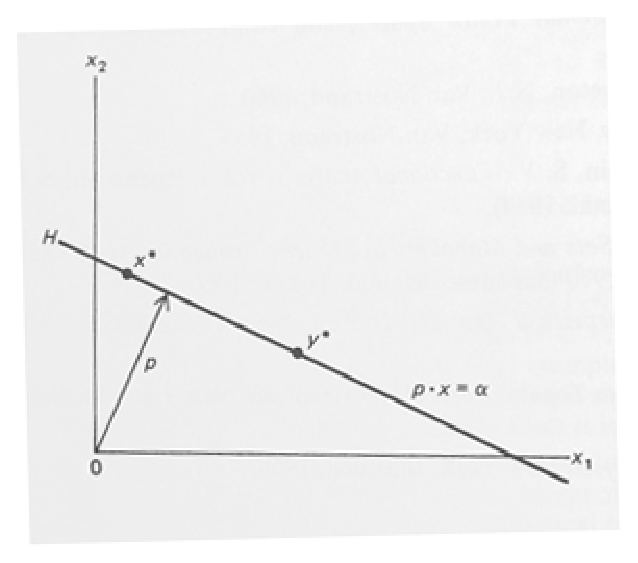
\includegraphics[width=0.47\textwidth]{line}}\hfill
\subfigure[Плоскость]{\includegraphics[width=0.47\textwidth]{3dplane}}
\caption{Примеры гиперплоскостей}\label{fig:Hplanes_exam}
\end{figure}

\begin{note}
Нетрудно проверить, что нормаль всегда ортогональна гиперплоскости.
Действительно, для любых $\vc{x}', \vc{x}'' \in \st{H}$ выполняется

\[\vc{p} \cdot (\vc{x}' - \vc{x}'')= \vc{p} \cdot \vc{x}' - \vc{p}
\cdot \vc{x}''=\gamma - \gamma =0.\]

\noindent В двумерном случае вектор $\vc{p}$ всегда перпендикулярен
прямой (см. Рис.~\ref{fig:Hplanes_exam} а)).
\end{note}

Изменяя значение $\gamma$ (сдвигая гиперплоскость), мы получаем
целое семейство гиперплоскостей. В двумерном случае это выглядит
следующим образом (см. Рис.~\ref{fig:hypermap}).

\input{pics/hypermap.TpX}


\begin{dfn}

\begin{enumerate}
\renewcommand{\theenumi}{(\asbuk{enumi})}

\item Пусть заданы два непустых множества $\st{X}$ и $\st{Y}$ в $\R^n$ и
гиперплоскость $\st{H}= \{ \vc{x}\in \R^n: \vc{p} \cdot \vc{x} =
\gamma\}$. Множества $\st{X}$ и $\st{Y}$ называются
\dw{отделимыми}\index{отделимые множества} гиперплоскостью $\st{H}$,
если $\vc{p} \cdot \vc{x} \leq \gamma$, для всех $\vc{x} \in
\st{X}$, и $\vc{p} \cdot \vc{y} \geq \gamma$, для всех $\vc{y} \in
\st{Y}$.

\item Если указанные неравенства выполняются как строгие ($\vc{p} \cdot \vc{x} < \gamma$
 для всех $\vc{x} \in \st{X}$ и $\vc{p} \cdot \vc{y} > \gamma$ для всех $\vc{y} \in
 \st{Y}$), то множества $\st{X}$ и $\st{Y}$ называют \dw{строго отделимыми}\index{строго отделимые множества}.
\end{enumerate}
\end{dfn}

Гиперплоскость $\st{H}$ в $\R^n$ разбивает $\R^n$ на два
\emph{полупространства} ${\{ \vc{x}: \vc{p} \cdot \vc{x} \leq
\gamma\}}$ и ${\{ \vc{x}: \vc{p} \cdot \vc{x} \geq \gamma\}}$.


\begin{dfn}

Гиперплоскость $\st{H}$ называется \dw{опорной} гиперплоскостью к
множеству $\st{X}$, если эта гиперплоскость имеет общую точку с
$\st{X}$, и множество $\st{X}$ полностью лежит в одном из замкнутых
полупространств, определяемых этой гиперплоскостью.\end{dfn}

Иллюстрация данного определения представлена на Рис.
\ref{fig:sup-hplane}. Здесь гиперплоскость имеет с множеством
$\st{X}$ общую точку $\vc{\hat x}$. В таком случае говорят, что
гиперплоскость является \dw{опорной в точке $\vc{\hat x}$}.

\input{pics/sup_hplane.TpX}

\begin{exer}
Докажите, что:
\begin{itemize}
  \item замкнутое полупространство является выпуклым множеством;
  \item гиперплоскость является замкнутым и выпуклым множеством.
\end{itemize}
\end{exer}

В классической математической экономике те задачи, которые сводятся
к максимизации или минимизации некоторых функций, обычно разрешаются
методами математического анализа. Основной прием, который при этом
используется, -- приравнивание производных нулю -- по существу
эквивалентен отысканию касательной, или опорной, гиперплоскости.
Суть дела здесь не в использовании аналитических методов, а в факте
существования указанных гиперплоскостей, на чем коренным образом
основывается решение многих таких задач.


\begin{teo}(Об отделяющей гиперплоскости, б/д)
\label{teo:sep-hplane}

Пусть $\st{X}$ --- непустое замкнутое выпуклое множество в $\R^n$.
Если точка $\vc{\hat x} \notin \st{X}$, то существует такой вектор
$\vc{p} \in \R^n$, $\vc{p} \neq \vc{0}$, и число $\gamma \in \R$,
что для любого $\vc{x} \in \st{X}$ выполняется:

\[\vc{p} \cdot \vc{x} \leq \gamma < \vc{p} \cdot \vc{\hat x}\]
\end{teo}

Фактически, речь идет о том, что множество  и точка $\vc{\hat x}$
лежат по разные стороны гиперплоскости $\vc{p} \cdot \vc{x} =
\gamma$ (см. Рис.~\ref{fig:sep-hplane} а)). Такая гиперплоскость
называется \dw{отделяющей}.

Тогда, утверждение теоремы можно переформулировать следующим
образом: \emph{для замкнутого выпуклого множества и любой не
принадлежащей ему точки существует отделяющая гиперплоскость}.

\begin{note}

Отметим, что на знаки компонентов вектора $\vc{p}$ ограничения не
накладываются, т.е. для вектора $\vc{p}$ может выполняться как
$\vc{p} \leq \vc{0}$, так и $\vc{p} \geq \vc{0}$, но не $\vc{p} =
\vc{0}$. Аналогично, $\gamma$ может быть больше, меньше, а кроме
того, и равно нулю.
\end{note}


\input{pics/sep_hplane.TpX}

В случае, когда $\vc{\hat x}$ является \emph{граничной} точкой
множества $\st{X}$ (см. Рис.~\ref{fig:sep-hplane} б)), можно
сформулировать следующее утверждение\footnote{См. также
раздел~\vref{app:topology} математического приложения.}.

\begin{teo}(Об опорной гиперплоскости, б/д)

Пусть $\vc{\hat x}$  --- граничная точка замкнутого выпуклого
множества $\st{X}$. Тогда существует опорная к $\st{X}$ в точке
$\vc{\hat x}$ гиперплоскость, т.е. существует такой вектор $\vc{p}
\in \R^n$, $\vc{p} \neq 0$, и число $\gamma \in \R$, что для любого
$x \in \st{X}$ выполняется $\vc{p} \cdot \vc{x} \leq \vc{p} \cdot
\vc{\hat x}$.
\end{teo}

\begin{note}
С другой стороны, это означает, что точка $\vc{\hat x}$ фактически
есть решение задачи:

\[
\left\{ \begin{array}{l}
 \vc{p} \cdot \vc{x} \rightarrow \max\\
 \vc{x} \in \st{X} \\
 \end{array} \right.
\]

Данное соображение понадобится нам ниже при обсуждении эффективных
точек множества.
\end{note}



\begin{teo}\label{teo:sep_hplane_Mink}(Минковского о
разделяющей гиперплоскости, б/д\/\footnote{\cite{Takayama:1985},
\cite{Braverman:1976}})

Пусть $\st{X}$ и $\st{Y}$ -- непустые, необязательно замкнутые,
выпуклые множества в пространстве $\R^n$, не имеющие общих точек
либо имеющие общими только граничные точки, и пусть хотя бы одно из
множеств, например, множество $\st{Y}$, имеет внутреннюю точку (т.е.
$\st{X} \cap \st{Y}^o = \emptyset$).

Тогда существует гиперплоскость, разделяющая эти два множества, т.е.
существует $\vc{p} \in \R^n$, $\vc{p} \neq \vc{0}$, и число $\gamma
\in \R$ такие, что для любого $\vc{x} \in \st{X}$ и любого $\vc{y}
\in \st{Y}$ выполняется соотношение:

\[
\vc{p} \cdot \vc{y} \leq \gamma \leq \vc{p} \cdot \vc{x}.
\]
\end{teo}

\input{pics/sep_sets.TpX}

Заметим, что в этом случае гиперплоскость называется
\dw{разделяющей}.

Утверждение данной теоремы проиллюстрировано на
Рис.~\ref{fig:sep-sets}. В случае \emph{б)} множества $\st{X}$ и
$\st{Y}$ имеют общую граничную точку.

\remrk{Единственность гиперплоскости в случае общей граничной
точки?}

Случай \emph{в)} демонстрирует существенность предположения о том,
что хотя бы одно из множеств должно иметь внутреннюю точку: в этом
случае множества $\st{X}$ и $\st{Y}$ не могут быть разделены.

\begin{exer}
Покажите на примерах, что для невыпуклых множеств это утверждения
трех теорем отделимости не имеют места.
\end{exer}


\begin{teo}(О строгой отделимости, б/д\/\footnote{\cite{Kapustin:2001} стр. 36})

Непустые, непересекающиеся множества $X$ и $Y$, по крайней мере одно
из которых ограничено, строго отделимы. \end{teo}

\section{Лемма Минковского-Фаркаша}

Одним из важнейших приложений теорем об отделимости является лемма
Минковского-Фаркаша, доказательство которой основывается на
соответствующих утверждениях. Однако предварительно мы сформулируем
еще одну лемму.

\begin{lem}

Пусть $\st{K}$ --- конус\index{конус} в пространстве $\R^n$ с
вершиной в нуле и пусть задан вектор $\vc{p} \in \R^n$. Если $\vc{p}
\cdot \vc{x}$ ограничено снизу для любого $\vc{x} \in \st{K}$, то
$\vc{p} \cdot \vc{x} \geq 0$ (для любого $\vc{x} \in \st{K}$).
\end{lem}

\remrk{В приложении дать определение конуса, многогранного выпуклого
конуса.}

\begin{proof}

По предположению об ограниченности $\vc{p} \cdot \vc{x}$, существует
число $\alpha \in \R$ такое, что $\vc{p} \cdot \vc{x} \geq \alpha$
для любого $\vc{x} \in \st{K}$. Поскольку $\st{K}$ является конусом
с вершиной в нуле, тот факт, что $\vc{x} \in \st{K}$ означает, что
$\theta \vc{x} \in \st{K}$ для любого $\theta \geq 0$. Тогда $\vc{p}
\cdot (\theta \vc{x}) \geq \alpha$ или $\vc{p} \cdot \vc{x} \geq
\alpha / \theta$ для любого $\vc{x} \in \st{K}$ и $\theta > 0$.
Рассматривая предел данного соотношения при $\theta \rightarrow
\infty$, получаем $\vc{p} \cdot \vc{x} \geq 0$.
\end{proof}


Сформулируем лемму Минковского-Фаркаша.

\begin{lem}(Минковского-Фаркаша)  \label{lem:MinkFarcas}

Пусть $\vc{a}^1, \vc{a}^2, \ldots, \vc{a}^l$ и $\vc{b}\neq0$ ---
векторы в пространстве $\R^n$. Предположим, что $\vc{b} \cdot \vc{x}
\geq 0$ для любых $\vc{x} \in \R^n$, таких, что $\vc{a}^k \cdot
\vc{x} \geq 0$, $k=1 \ldots l$. Тогда существуют неотрицательные
числа $\lambda_1, \lambda_2, \ldots, \lambda_l$, одновременно не
равные нулю, такие, что $\vc{b}=\sum\limits_{k=1}^l{\lambda_k
\vc{a}^k}$.
\end{lem}

\begin{proof}

Пусть $\st{K}$ --- многогранный выпуклый конус, порожденный
векторами $\vc{a}^1, \vc{a}^2, \ldots, \vc{a}^l$. Тогда $\st{K}$
является замкнутым множеством (\remrk{Почему?}). Необходимо
показать, что $\vc{b} \in \st{K}$.

Предположим, что $\vc{b} \notin \st{K}$. Тогда $\st{K}$ ---
непустое, замкнутое, выпуклое множество, не включающее точку
$\vc{b}$. Тогда, по Теореме \ref{teo:sep-hplane}, существует такой
вектор $\vc{p} \in \R^n$, $\vc{p} \neq 0$, и число $\alpha \in \R$,
что для любого $\vc{x} \in \st{K}$ выполняется\footnote{Знаки
неравенств в утверждении теоремы можно одновременно изменить на
противоположные}:

\[\vc{p} \cdot \vc{x} \geq \alpha > \vc{p} \cdot \vc{b}.\]

Таким образом, $\vc{p} \cdot \vc{x}$ ограничено снизу для любого
$\vc{x} \in \st{K}$. По предыдущей лемме получаем $\vc{p} \cdot
\vc{x} \geq 0$ для любого $\vc{x} \in \st{K}$. Кроме того, поскольку
$\vc{0} \in \st{K}$, $\vc{p} \cdot \vc{0} \geq \alpha$ или $\alpha
\leq 0$. Отсюда $\vc{p} \cdot \vc{b} < 0$.

Поскольку $\vc{a}^k \in \st{K}$, то $\vc{p} \cdot \vc{a}^k \geq 0$,
$k=1 \ldots l$. Тогда для найденного вектора $\vc{p}$ получаем
$\vc{b} \cdot \vc{p} < 0$ при $\vc{p} \cdot \vc{a}^k \geq 0$, $k=1
\ldots l$. Это противоречит условию теоремы. Значит, $\vc{b} \in
\st{K}$. По свойству многогранного выпуклого конуса, это означает,
что существуют неотрицательные числа $\lambda_1, \lambda_2, \ldots,
\lambda_l$, такие, что $\vc{b}=\sum\limits_{k=1}^l{\lambda_k
\vc{a}^k}$. Поскольку $\vc{b}\neq0$, числа $\lambda_1, \lambda_2,
\ldots, \lambda_l$ не могут быть одновременно равны нулю.


\end{proof}


\begin{note}(к лемме Минковского-Фаркаша)

\begin{enumerate}
\renewcommand{\theenumi}{(\alph{enumi})}

  \item Если $b=0$, то допускается одновременное равенство нулю всех
  $\lambda_k$, $k=1 \ldots l$.

  \item Верно и обратное утверждение относительно Леммы \ref{lem:MinkFarcas},
  а именно, если $\vc{a}^1, \vc{a}^2, \ldots, \vc{a}^l$ и $\vc{b}\neq0$
  ---  векторы в пространстве $\R^n$ и существуют неотрицательные
   коэффициенты $\lambda_1, \lambda_2, \ldots, \lambda_l$,
   одновременно не равные нулю, такие, что $\vc{b}=\sum\limits_{k=1}^l{\lambda_k
   \vc{a}^k}$,то $\vc{b} \cdot \vc{x} \geq 0$ для любых $\vc{x} \in \R^n$, таких,
   что $\vc{a}^k \cdot \vc{x} \geq 0$, $k=1 \ldots l$.

\end{enumerate}

\end{note}


\remrk{Можно добавить векторно-матричную и геометрическую
интерпре\-тацию леммы из \cite{Takayama:1985}, стр. 47.}

Лемма Минковского-Фаркаша играет важную роль в теории линейного
программирования, теории игр, теории нелинейного программирования и
т.д.

\newpage

\section{Эффективные точки на выпуклых
множествах\protect\footnote{\cite{Takayama:1985}}}

Особую роль в экономическом анализе играют эффективные точки
различных множеств. Можно ввести следующие определения.

\begin{dfn}

Пусть $\st{X} \subset \R^n$ --- некоторое замкнутое множество.

\begin{enumerate}
  \item Точка ${\vc{\hat x}} \in \st{X} $ называется (\textbf{строго}) \textbf{эффективной
точкой} этого множества, если не существует другой точки $\vc{x} \in
\st{X}$, такой, что $\vc{x} \geq \vc{\hat x}$.

  \item Точка $\vc{\tilde x} \in \st{X}$ называется \textbf{слабо эффективной} точкой
множества~$\st{X}$, если не существует другой точки $\vc{x} \in
\st{X}$, такой, что $\vc{x} \gg \vc{\tilde x}$.

\end{enumerate}
\end{dfn}

Из приведенного выше определения нетрудно видеть, что любая
эффективная точка является и слабо эффективной. С другой стороны,
если точка не является слабо эффективной, то она не может быть и
строго эффективной.

\begin{comm}
Проиллюстрируем идею эффективной точки множества на простом примере.
Классический пример выпуклого множества, приводимый в элементарных
учебниках по экономической теории --- множество производственных
возможностей страны, ограниченное \dw{кривой производственных
возможностей} (англ., \emph{production possibility
frontier}\footnote{\cite{McConnell:1996}}). Кривая производственных
возможностей представлена на Рис.~\ref{fig:ppfrontier}.

Стандартно предполагается, что при ограниченных запасах факторов
производства, в экономике производятся два вида товаров: пушки и
масло. Все сочетания пушек и масла на кривой производственных
возможностей представляют максимальные их количества, которые могут
быть получены лишь в результате наиболее эффективного использования
всех имеющихся ресурсов.

Чтобы осуществить производство различных комбинаций пушек и масла,
представленных на графике, общество должно обеспечить полную
занятость ресурсов и полный объем производства. Таким образом,
каждая точка на кривой производственных возможностей представляет
собой какой-то максимальный объем производства двух указанных
товаров.

\input{pics/ppfrontier.TpX}

Эффективная точка есть граничная точка множества производственных
возможностей $\st{X}$. Действительно, как видно на
Рис.~\ref{fig:ppfrontier} \emph{а)}, точка $\vc{\hat x}$ является
\emph{эффективной}, поскольку все точки $\vc{x}$, такие, что $\vc{x}
\geq \vc{\hat x}$ (т.\/е. точки, находящиеся выше и правее $\vc{\hat
x}$), не принадлежат множеству $\st{X}$. По аналогичным соображениям
точка $\vc{\bar x}$ эффективной не является.

Следует отметить, что эффективная точка множества производственных
возможностей представляет собой такую комбинацию затрат-выпуска, что
невозможно увеличить выпуск по одного из товаров, не уменьшив
выпуска другого товара или не увеличив расход ресурсов.

На Рис.~\ref{fig:ppfrontier} \emph{б)} приведен пример \emph{слабо
эффективной} точки. Если предположить, что кривая производственных
возможностей страны имеет линейные горизонтальный и вертикальный
участки ($AB$ и $CD$ соответственно), как показано на рисунке, то
точки, лежащие на этих участках, являются слабо эффективными.

Действительно, точка $\vc{\tilde x}$ является слабо эффективной,
поскольку не существует другой точки $\vc{x}$, лежащей в множестве
$\st{X}$, такой, что $\vc{x} \gg \vc{\tilde x}$.

\end{comm}


Сформулируем следующие фундаментальные теоремы.

\begin{teop}(Условия эффективности точки)\label{teo:1_fund_production}

Пусть $\st{X} \subset \R^n$ --- некоторое (замкнутое) множество.
Пусть $\vc{\hat x}$ есть решение задачи:

\begin{equation}\label{eq:eff_conditions}
\left\{ \begin{array}{l}
 \vc{p} \cdot \vc{x} = p_1x_1 + \ldots + p_n x_n\to \max  \\
 \vc{x} \in \st{X} \\
 \end{array} \right.
\end{equation}


\begin{enumerate}
\renewcommand{\theenumi}{(\roman{enumi})}
  \item Если $\vc{p} \geq \vc{0}$, то точка $\vc{\hat x} \in \st{X}$ является
  слабо эффективной.
  \item Если $\vc{p} \gg \vc{0}$, то точка $\vc{\hat x} \in \st{X}$ является
  эффективной.
\end{enumerate}

\end{teop}

\begin{proof}(От противного)

(i) Предположим, что утверждение данного пункта не выполняется. В
этом случае существует $\vc{\bar x} \in \st{X}$ такой, что $\vc{\bar
x} \gg \vc{\hat x}$. Тогда, поскольку $\vc{p} \geq \vc{0}$, получаем
$\vc{p} \cdot \vc{\bar x} > \vc{p} \cdot \vc{\hat x}$. Однако это
противоречит тому факту, что $\vc{\hat x}$ есть решение задачи
(\ref{eq:eff_conditions}).

(ii) Докажите самостоятельно в качестве \textbf{упражнения}.

\end{proof}



Отметим, что в приведенных теоремах не накладывается никаких условий
на множество $\st{X}$. Обратное утверждение требует более сильных
предположений относительно устройства множества $\st{X}$, а именно,
выпуклости этого множества. Для доказательства обратного утверждения
потребуется следующая лемма.

\begin{lem}

Пусть $\st{X} \subset \R^n$ --- некоторое замкнутое множество. Если
$\vc{\hat x}$ является слабо эффективной точкой множества $\st{X}$,
то $\st{X} \cap \st{Z}^o=\emptyset$, где $\st{Z}^o=\{\vc{z} \in
\R^n: \vc{z} \gg \vc{\hat x}\}$.\end{lem}

\begin{proof}(От противного)

Предположим, что утверждение леммы не выполняется. Тогда существует
$\vc{z} \in \st{X}$ такой, что $\vc{z} \gg \vc{\hat x}$. Тогда
$\vc{\hat x}$ не является (слабо) эффективной точкой множества
$\st{X}$, что противоречит предположению леммы.

\end{proof}

\begin{exer}
Докажите, что если  $\vc{\hat x}$ является строго эффективной точкой
множества $\st{X}$, то $\st{X} \cap \st{Z}=\{\vc{\hat x}\}$, где
$\st{Z}=\{\vc{z}\in \R^n: \vc{z} \geqq \vc{\hat x}\}$.
\end{exer}

\begin{exer}
Докажите, что в обоих случаях множество $\st{Z}$ является выпуклым.
\end{exer}

\begin{teop}(Свойство слабо эффективной точки)\label{teo:2_fund_production}

Пусть $\st{X} \subset \R^n$ --- выпуклое и замкнутое множество. Если
точка ${\vc{\hat x} \in \st{X}}$ является слабо эффективной точкой
множества $\st{X}$, то существует вектор ${\vc{p} \geq \vc{0}}$,
$\vc{p} \in \R^n$, такой, что $\vc{p} \cdot \vc{\hat x} \geq \vc{p}
\cdot \vc{x}$ для любых $\vc{x} \in \st{X}$, т.е. $\vc{\hat x}$ есть
решение задачи (\ref{eq:eff_conditions}).
\end{teop}

\begin{proof}

Пусть $\st{Z}=\{\vc{z}\in \R^n: \vc{z} \geqq \vc{\hat x}\}$.

Тогда $\st{Z}^o=\{\vc{z} \in \R^n: \vc{z} \gg \vc{\hat x}\} \neq
\emptyset$. Множество $\st{Z}^o$ является выпуклым. Поскольку
$\vc{\hat x}$ является слабо эффективной точкой множества $\st{X}$,
то, по предыдущей лемме, $\st{X} \cap \st{Z}^o=\emptyset$. Таким
образом, имеем два непересекающихся множества, внутренность по
крайней мере одного из которых непуста.

Значит, по теореме отделимости Минковского
(Теорема~\ref{teo:sep_hplane_Mink}), найдутся $\vc{p} \in \R^n$,
$\vc{p}\neq \vc{0}$, и число $\gamma \in \R$ такие, что для любого
$\vc{x} \in \st{X}$ и любого $\vc{z} \in \st{Z}^o$ выполняется
соотношение:

\[
\vc{p} \cdot \vc{x} \leq \gamma \leq \vc{p} \cdot \vc{z}.
\]

Отметим, что $\gamma = \vc{p} \cdot \vc{\hat x}$. Действительно,
поскольку $\vc{\hat x} \in \st{X}$, то $\gamma \geq \vc{p} \cdot
\vc{\hat x}$. С другой стороны, $\gamma \leq \vc{p} \cdot \vc{\hat
x}$. Действительно, если это не так, то $\vc{p} \cdot \vc{z}\geq
\gamma> \vc{p} \cdot \vc{\hat x}$ должно выполняться для любого
$\vc{z} \in \st{Z}^o$. Однако, это невозможно: мы всегда можем
подобрать такое $\vc{\bar z}$, что $\vc{p}\cdot\vc{\bar z}<\gamma$.
Отсюда следует, что $\gamma = \vc{p} \cdot \vc{\hat x}$.

Кроме того, $\vc{p} \geq \vc{0}$ (если это не так, то найдется такая
компонента ${p_i < 0}$ вектора $\vc{p}$, что, подобрав достаточно
большую по значению компоненту $z_i$ вектора $\vc{z}$, мы получим
$\vc{p} \cdot \vc{z}<\vc{p} \cdot \vc{\hat x}$, что является
противоречием).

Таким образом, мы получили, что для любого $\vc{x} \in \st{X}$
выполняется $\vc{p} \cdot \vc{x} \leq \vc{p} \cdot \vc{\hat x}$,
причем $\vc{p} \geq \vc{0}$.
\end{proof}

\begin{note}
\begin{enumerate}
  \item Если множество $\st{X}$ является многогранным выпуклым конусом, то в
условиях сформулированной выше теоремы можно показать, что $\vc{p}
\gg \vc{0}$. Вообще говоря, только в этом случае можно утверждать,
что точка $\vc{\hat x}$ является строго эффективной.

  \item Напомним, что всякая строго эффективная точка
  является и слабо эффективной. В общем же случае нельзя сформулировать
  условия подобного рода для строгой эффективности точки.

  Действительно, из того факта, что точка
  является эффективной, вовсе не следует, что $\vc{p} \gg \vc{0}$. В
  качестве примера на Рис.~\ref{fig:circle_eff} приведем окружность (выпуклое
  множество), точка $A$ которой очевидным образом является
  эффективной, но $\vc{p} \geq \vc{0}$. (В качестве \textbf{упражнения}
  аккуратно докажите этот факт).

\input{pics/circle_eff.TpX}

\end{enumerate}


\end{note}


\begin{comm}

Теоремы ~\ref{teo:1_fund_production} и \ref{teo:2_fund_production}
позволяют описать идею эффективной точки множества с точки зрения
задачи максимизации, а именно, с учетом доказанного в теореме
утверждения, можно говорить о том, что любая эффективная точка
множества $\st{X}$ есть, при некотором $\vc{p} \geq \vc{0}$, решение
следующей задачи:

\[
\left\{ \begin{array}{l}
 \vc{p} \cdot \vc{x} \to \max  \\
 \vc{x} \in \st{X} \\
 \end{array} \right.
\]

Данное соображение поддается прозрачной экономической интерпретации.
Если в рассматриваемом нами примере про кривую производственных
возможностей страны точка $\vc{\hat x}$ является эффективной, и
страна \emph{фактически} производит указанный набор товаров
$\vc{\hat x}=(\hat x_1, \hat x_2)$, то можно утверждать, что в
данной точке национальный доход:

\[
I = \vc{p} \cdot \vc{\hat x}= p_1\hat x_1 + p_2 \hat x_2
\]

\noindent достигает своего максимума. При этом, вектор $\vc{p} \geq
\vc{0}$ трактуется как вектор цен на соответствующие товары.

Иллюстрация данной идеи представлена на Рис.~\ref{fig:ppfront_max}.

\input{pics/ppfront_max.TpX}

\end{comm}


\newpage

\section{Оптимальность по
Парето\protect\footnote{[Конспект ЕУ по математике]}}

Рассмотрим $\st{X} \subset \R^n$ и набор функций $f_1(\vc{x}),
f_2(\vc{x}), \ldots, f_m(\vc{x})$.

\begin{dfn}(Доминирование по Парето)

\begin{enumerate}
\item Будем говорить, что точка $\vc{\tilde x} \in \st{X}$ \dw{доминирует} точку
$\vc{\hat x} \in \st{X}$ \dw{по Парето}, если $f_j(\vc{\tilde x})
\geq f_j(\vc{\hat x})$, $j=1 \ldots m$, и хотя бы одно из этих
неравенств выполняется, как строгое.

\item Будем говорить, что точка $\vc{\tilde x}$ \dw{строго доминирует} точку
$\vc{\hat x}$ \dw{по Парето}, если $f_j(\vc{\tilde x}) >
f_j(\vc{\hat x})$, $j=1 \ldots m$.
\end{enumerate}
\end{dfn}

\begin{dfn}(Оптимальность по Парето)

\begin{enumerate}

\item Будем говорить, что точка $\vc{\hat x} \in \st{X}$ является \dw{оптимальной
по Парето}, если $\nexists \,{\vc{\tilde x}} \in \st{X}$, такой, что
точка $\vc{\tilde x}$ доминирует точку $\vc{\hat x}$ по Парето.

\item Будем говорить, что точка $\vc{\hat x} \in \st{X}$ является \dw{слабо
оптимальной по Парето}, если $\nexists \,{\vc{\tilde x}} \in
\st{X}$, такой, что точка $\vc{\tilde x}$ строго доминирует точку
$\vc{\hat x}$ по Парето.

\end{enumerate}
\end{dfn}

Сформулируем следующие важные теоремы.

\begin{teop}\label{teo:Pareto_opt_conditions}(Условия оптимальности точки)

Пусть $\st{X}$ --- замкнутое множество, и $\vc{\hat x} \in \st{X}$
есть решение задачи:

\[ \left\{
\begin{array}{l}
 p_1 f_1 (\vc{x}) + p_2 f_2 (\vc{x}) + \ldots + p_m f_m (\vc{x})\to \max  \\
 \vc{x} \in \st{X} \\
 \end{array} \right.
\]

\begin{enumerate}
\renewcommand{\theenumi}{(\roman{enumi})}

\item Если коэффициенты $p_j$, $j=1 \ldots m$, неотрицательны и одновременно не равны нулю,
т.е. $\vc{p} \geq \vc{0}$, то $\vc{\hat x}$ будет слабо оптимальной
по Парето точкой.

\item Если $p_j > 0$, $j=1 \ldots m$, т.е. $\vc{p} \gg \vc{0}$, то $\vc{\hat x}$ ---
оптимальная по Парето точка.

\end{enumerate}
\end{teop}

\begin{proof}
Доказательство данной теоремы выполните в качестве
\textbf{упражнения}.
\end{proof}

Для доказательства следующей теоремы нам потребуется следующая
Фундаментальная лемма.


\begin{lemp}(Фундаментальная лемма)

Пусть $\st{X}$ --- выпуклое замкнутое множество, а заданные на нем
функции $f_1(\vc{x}), f_2(\vc{x}), \ldots, f_m(\vc{x})$ --- вогнуты
($f_j: \st{X} \rightarrow \R$, $j=1 \ldots m$). Пусть числа $b_1,
b_2, \ldots, b_m$ таковы, что система неравенств

\[
\left\{ \begin{array}{l}
 f_1(\vc{x}) > b_1\\
 f_2(\vc{x}) > b_2 \\
  \cdots  \\
 f_m(\vc{x}) > b_m \\
 \end{array} \right.
\]

\noindent не имеет решения ни для какого $\vc{x} \in \st{X}$.

Тогда существуют такие неотрицательные коэффициенты $p_1, p_2,
\ldots, p_m$, не все одновременно равные нулю, что для любого
$\vc{x} \in \st{X}$ выполняется соотношение:

\begin{equation}\label{eq:ineq_fund_lemma}
p_1 f_1(\vc{x}) + p_2 f_2(\vc{x}) + \ldots + p_m f_m(\vc{x}) \leq
p_1 b_1 + p_2 b_2 + \ldots + p_m b_m.
\end{equation}

\end{lemp}

\remrk{Связь с Фаркашем?}

\begin{proof}

Для каждой точки $\vc{x} \in \st{X}$ определим множество
${\st{Z}_{\vc{x}} \subset \R^m}$ следующим образом:

\[
\st{Z}_{\vc{x}}=\{\vc{z}\in \R^m: z_1\leq f_1(\vc{x}), z_2\leq
f_2(\vc{x}), \ldots, z_m\leq f_m(\vc{x})\}.
\]

Обозначим $\st{Z}= \mathop \cup \limits_{\vc{x} \in \st{X}}
\st{Z}_{\vc{x}}$.

Отметим, что множество $\st{Z}$ является выпуклым. Действительно,
возьмем точки $\vc{z'} \in \st{Z}_{\vc{x'}}$ и $\vc{z''} \in
\st{Z}_{\vc{x''}}$ (очевидно, что $\vc{z'}, \vc{z''} \in \st{Z}$) и
число $\theta \in \R$, $0 \leq \theta \leq 1$. Тогда для всех $j=1
\ldots m$ выполняется:

\[
\bar{z}_{j}= \theta z'_j + (1- \theta) z''_j\leq  \theta
f_j(\vc{x'}) + (1- \theta) f_j(\vc{x''}) \leq  f_j(\theta\vc{x'} +
(1- \theta) \vc{x''})=f_j(\vc{\bar x}),
\]

\noindent где $\vc{\bar x}=\theta\vc{x'} + (1- \theta) \vc{x''} \in
\st{X}$, а последнее неравенство справедливо в силу вогнутости
функций $f_j$. Тогда

\[
\vc{\bar z} = \left( {\begin{array}{*{20}c}
   \bar{z}_1  \\
   \bar{z}_2  \\
    \vdots   \\
   \bar{z}_m  \\
\end{array}} \right) \in \st{Z}_{\vc{\bar x}} \subset \st{Z},
\]

\noindent что доказывает выпуклость множества $\st{Z}$.

Далее, отметим, что точка $\vc{b} =(b_1, b_2, \ldots, b_m)\notin
\st{Z}$. Действительно, если бы $\vc{b} \in \st{Z}$, то нашелся бы
такой вектор $\vc{\tilde x} \in \st{X}$, что $\vc{b} \in
\st{Z}_{\vc{\tilde x}}$, а значит, $f_j(\vc{\tilde x}) \geq b_j$ для
всех $j=1 \ldots m$, что противоречит условию леммы.

Тогда, по Теореме~\ref{teo:sep-hplane}, множество $\st{Z}$ и точка
$\vc{b}$ отделимы, т.\,е. существует такой вектор $\vc{p} \in \R^m$,
$\vc{p} \neq \vc{0}$, что для любого $\vc{z} \in \st{Z}$

\begin{equation}\label{eq:ineq1_fundlemma}
\vc{p} \cdot \vc{z} \leq \vc{p} \cdot \vc{b}.
\end{equation}

Преобразуя данное неравенство, получаем:

\begin{equation}\label{eq:ineq2_fundlemma}
\vc{p} \cdot (\vc{z} - \vc{b}) \leq 0.
\end{equation}


Поскольку, очевидно, $\vc{z} \leq \vc{b}$ для любого $\vc{z} \in
\st{Z}$, то любая из компонент вектора $(\vc{z} - \vc{b})$ может
принимать сколь угодно большие отрицательные значения. Это в свою
очередь означает, что, для выполнения
неравенства~(\ref{eq:ineq2_fundlemma}), все компоненты вектора
$\vc{p}$ должны быть неотрицательны.

Раскрывая неравенство~(\ref{eq:ineq1_fundlemma}) с учетом
определения множества $\st{Z}_{\vc{x}}$, получаем, что для любого
$\vc{x}\in \st{X}$ существует такой вектор $\vc{p}\geq \vc{0}$, что

\begin{multline}
p_1 z_1 + p_2 z_2 + \ldots + p_m z_m \leq p_1 f_1(\vc{x}) + p_2
f_2(\vc{x}) + \ldots + p_m f_m(\vc{x}) \leq {}\\ \leq p_1 b_1 + p_2
b_2 + \ldots + p_m b_m.
\end{multline}


Последняя часть полученного неравенства доказывает утверждение
леммы.

\end{proof}

Теперь мы можем приступить к доказательству следующего важного
свойства слабо оптимальной точки.

\begin{teop}(Свойство слабо оптимальной
по Парето точки)

Пусть $\st{X}$ --- замкнутое выпуклое множество в $\R^n$. Пусть
заданы вогнутые функции $f_1(\vc{x}), f_2(\vc{x}), \ldots,
f_m(\vc{x}): \st{X} \to \R$.

Если $\vc{\hat x} \in \st{X}$ является слабо оптимальной по Парето
точкой, то существуют неотрицательные коэффициенты $p_1, p_2,
\ldots, p_m$, не все одновременно равные нулю, такие, что $\vc{\hat
x}$ представляет собой решение задачи:

\[ \left\{
\begin{array}{l}
 p_1 f_1(\vc{x}) + p_2 f_2(\vc{x}) + \ldots + p_m f_m(\vc{x})\to \max  \\
 \vc{x} \in \st{X} \\
 \end{array} \right.
\]
\end{teop}

\begin{proof}

Обозначим
\begin{align*}
 b_1 &=f_1(\vc{\hat x}),\\
 b_2 &=f_2(\vc{\hat x}),\\
  &\cdots \\
 b_m &=f_m(\vc{\hat x}).
\end{align*}

Поскольку $\vc{\hat x}$ является слабо оптимальной по Парето точкой,
это означает, что $\nexists \, \vc{\tilde x} \in \st{X}:
f_j(\vc{\tilde x})> f_j(\vc{\hat x})$, $j=1 \ldots m$.

Другими словами, с учетом введенных обозначений, система неравенств

\[
\left\{ \begin{array}{l}
 f_1(\vc{x}) > b_1\\
 f_2(\vc{x}) > b_2 \\
  \cdots  \\
 f_m(\vc{x}) > b_m \\
 \end{array} \right.
\]

\noindent не имеет решения ни при каком $\vc{x} \in \st{X}$.

Тогда, в соответствии с утверждением доказанной выше Фундаментальной
леммы, существуют неотрицательные коэффициенты $p_1, p_2, \ldots,
p_m$, не все одновременно равные нулю, такие, что для любого $\vc{x}
\in \st{X}$ выполняется соотношение:

\begin{multline}
p_1 f_1(\vc{x}) + p_2 f_2(\vc{x}) + \ldots + p_m f_m(\vc{x}) \leq
p_1 b_1 + p_2 b_2 + \ldots + p_m b_m = \\ = p_1 f_1(\vc{\hat x}) +
p_2 f_2(\vc{\hat x}) + \ldots + p_m f_m(\vc{\hat x}).
\end{multline}

\noindent  Отсюда получаем, что
\[p_1 f_1(\vc{x}) + p_2 f_2(\vc{x}) + \ldots + p_m
f_m(\vc{x}) \leq p_1 f_1(\vc{\hat x}) + p_2 f_2(\vc{\hat x}) +
\ldots + p_m f_m(\vc{\hat x}). \]

\noindent Это означает, что точка $\vc{\hat x}$ представляет собой
решение задачи:

\[ \left\{
\begin{array}{l}
 p_1 f_1(\vc{x}) + p_2 f_2(\vc{x}) + \ldots + p_m f_m(\vc{x})\to \max  \\
 \vc{x} \in \st{X} \\
 \end{array} \right.
\]


\end{proof}



\section{Общая теорема Куна-Таккера}

\begin{dfn}
Задача максимизации вогнутой функции на выпуклом (замкнутом?)
множестве называется \dw{задачей выпуклого программирования}.
\end{dfn}

Формально, задачу выпуклого программирования можно записать
следующим образом:

\begin{equation}\label{problem:ZVPG}
\left\{ \begin{array}{l}
 f_0(\vc{x}) \to \max  \\
 \vc{x} \in \st{G} \\
 \end{array} \right.
\end{equation}

\noindent где $\st{G}=\{\vc{x} \in \st{X}:  f_j (\vc{x}) \geq b_j, j
= 1 \ldots m \}$, $\st{X}$ --- выпуклое и замкнутое множество, а
функции $f_0(\vc{x}), f_1(\vc{x}), \ldots, f_m(\vc{x})$ ---
вогнутые.

\begin{exer}
Покажите, что множество $\st{G}$ является выпуклым и замкнутым.
\end{exer}

Отметим, что если $\st{X}\equiv \R^n$, то
задача~(\ref{problem:ZVPG}) называется \dw{основной (общей) задачей
выпуклого программирования}. Для удобства
задачу~(\ref{problem:ZVPG}) часто записывают в виде:

\begin{equation}\label{problem:ZVP}
\left\{ \begin{array}{l}
 f_0(\vc{x}) \to \max  \\
 f_j (\vc{x}) \geq b_j, j = 1 \ldots m\\
 \vc{x} \in \st{X} \\
 \end{array} \right.
\end{equation}

Часто в литературе ограничения на функции $f_j(\vc{x})$ записывают в
виде $f_j (\vc{x}) \geq 0$. Отметим, что постановка
задачи~(\ref{problem:ZVP}) не противоречит данному подходу.
Действительно, перенося $b_j$ в левые части ограничений-неравенств,
получаем, $g_j (\vc{x})=f_j (\vc{x}) - b_j\geq 0$, где функции $g_j
(\vc{x})$ по-прежнему являются вогнутыми, поскольку вычитание или
прибавление константы к вогнутой функции не влияет на ее вогнутость.
Здесь и далее мы будем придерживаться обозначений, введенных для
задачи~(\ref{problem:ZVP}).

Продолжая тему оптимальности по Парето из предыдущего раздела,
отметим следующий важный факт.

\begin{prop}\label{prop:x_weakoptimal}
Если $\vc{\hat x}$ есть решение задачи~(\ref{problem:ZVP}), то
$\vc{\hat x}$ --- слабо оптимальная по Парето точка относительно
набора функций $f_0, f_1, \ldots, f_m$.
\end{prop}

\begin{proof}(От противного)

Пусть $\vc{\hat x}$ не является слабо оптимальной по Парето точкой.
Тогда $\exists \,\vc{\tilde x} \in \st{X}$, такая, что

\[
\left\{ \begin{array}{l}
 f_0(\vc{\tilde x}) > f_0(\vc{\hat x})\\
 f_1(\vc{\tilde x}) > f_1(\vc{\hat x})\\
  \cdots  \\
 f_m(\vc{\tilde x}) > f_m(\vc{\hat x}) \\
 \end{array} \right.
\]

\noindent Таким образом, с одной стороны $\vc{\tilde x}\in \st{X}$
удовлетворяет ограничениям задачи ($f_j(\vc{\tilde x}) >
f_j(\vc{\hat x})\geq b_j$, $j=1 \ldots m$), а с другой стороны,
${f_0(\vc{\tilde x}) > f_0(\vc{\hat x})}$. Это означает, что
$\vc{\hat x}$ не является решением задачи~(\ref{problem:ZVP}).
Получили противоречие. Значит, $\vc{\hat x}$ является слабо
оптимальной по Парето точкой.
\end{proof}



\begin{exer}
Укажите, при каких условиях решение задачи~(\ref{problem:ZVP}) есть
строго оптимальная по Парето точка.
\end{exer}


\subsection{Понятие условий регулярности}

В утверждениях данного раздела нам понадобится ввести некоторые
предположения об устройстве множества $\st{X}$ --- так называемые
\dw{условия регулярности} множества.

\begin{dfn}(Обычная регулярность, Карманов, стр. 50)

Если для любого $j=1 \ldots m$ существует такая точка $\vc{x}_j \in
\st{X}$, что

\[
 f_j(\vc{x}_j) > b_j,\\
\]

\noindent то говорят, что множество $\st{X}$ удовлетворяет условию
регулярности.

\end{dfn}



\begin{dfn}(Регулярность по Слейтеру)

Если в множестве $\st{X}$ существует такой вектор $\vc{\bar x}$, для
которого при произвольных $b_1, \ldots, b_m$ выполняется:

\[
\left\{ \begin{array}{l}
 f_1(\vc{\bar x}) > b_1\\
 f_2(\vc{\bar x}) > b_2 \\
  \cdots  \\
 f_m(\vc{\bar x}) > b_m \\
 \end{array} \right.
\]

\noindent то говорят, что множество $\st{X}$ \dw{регулярно по
Слейтеру} (или для него выполняется \dw{условие Слейтера}).

\end{dfn}

\begin{dfn} (Регулярность по Карлину)

Множество $\st{X}$ является \dw{регулярным по Карлину}, если для
любого вектора $\vc{p} \geq \vc{0}$ и произвольных $b_1, \ldots,
b_m$ существует такой вектор $\vc{\bar x} \in \st{X}$, что:
\[
p_1 f_1(\vc{\bar x}) + p_2 f_2(\vc{\bar x}) + \ldots + p_m
f_m(\vc{\bar x}) > p_1 b_1 + p_2 b_2 + \ldots + p_m b_m.
\]

\end{dfn}

\begin{exer}
Проверьте, что все три условия регулярности эквивалентны.
\end{exer}


\subsection{Предварительные предложения}

Сформулируем следующее предложение.

\begin{prop}\label{prop:necessity_TKT}

Пусть $\st{X}$ --- выпуклое множество в $\R^n$. Пусть заданы
вогнутые функции $f_0, f_1, f_2, \ldots, f_m: \st{X} \to \R$. Пусть
$\vc{\hat x}$ есть решение задачи~(\ref{problem:ZVP}).

Тогда существуют неотрицательные коэффициенты $p_0, p_1, \ldots,
p_m$, не все одновременно равные нулю, такие, что $\vc{\hat x}$ есть
решение задачи:

\[
\left\{ \begin{array}{l}
 p_0 f_0(\vc{x}) + p_1 f_1(\vc{x})+ \ldots + p_m f_m(\vc{x}) \to \max  \\
 \vc{x} \in \st{X} \\
 \end{array} \right.
\]

\end{prop}

\begin{proof}
Доказательство этого утверждения мгновенно вытекает из свойства
слабо оптимальной по Парето точки.

Действительно, поскольку $\vc{\hat x}$ есть решение
задачи~(\ref{problem:ZVP}), то, по
Предложению~\ref{prop:x_weakoptimal}, $\vc{\hat x}$ является слабо
оптимальной по Парето точкой. Тогда, по свойству слабо оптимальной
точки (Теорема~\ref{teo:property_weak_optimal}), найдутся
неотрицательные коэффициенты $p_0, p_1, p_2, \ldots, p_m$, не все
одновременно равные нулю, такие, что $\vc{\hat x}$ есть решение
задачи:

\[
\left\{ \begin{array}{l}
 p_0 f_0(\vc{x}) + p_1 f_1(\vc{x})+ \ldots + p_m f_m(\vc{x}) \to \max  \\
 \vc{x} \in \st{X} \\
 \end{array} \right.
\]

\end{proof}

Отметим, что сформулированное выше утверждение верно и в обратную
сторону. Однако, при этом, не требуется выпуклость множества
$\st{X}$.

\begin{prop}\label{prop:sufficiency_TKT}

Пусть заданы вогнутые функции $f_0, f_1, f_2, \ldots, f_m: \st{X}
\to \R$. Пусть ${\vc{\hat x} \in \st{X}}$ есть решение задачи:

\[
\left\{ \begin{array}{l}
 f_0(\vc{x}) + p_1 f_1(\vc{x})+ \ldots + p_m f_m(\vc{x}) \to \max  \\
 \vc{x} \in \st{X} \\
 \end{array} \right.
\]

\noindent где $p_1,p_2 \ldots, p_m$ --- неотрицательные
коэффициенты, не все одновременно равные нулю.

Тогда $\vc{\hat x}$ есть решение задачи~(\ref{problem:ZVP}) для
некоторых (каких?) $b_1, b_2, \ldots, b_m$.

\end{prop}

\begin{proof}
Доказательство данного утверждения вытекает из условия оптимальности
по Парето (Теорема~\ref{teo:Pareto_opt_conditions}). Действительно,
положив $p_0=1$, заметим, что $\vc{\hat x}$ есть решение задачи:

\[
\left\{ \begin{array}{l}
 p_0 f_0(\vc{x}) + p_1 f_1(\vc{x})+ \ldots + p_m f_m(\vc{x}) \to \max  \\
 \vc{x} \in \st{X}, \\
 \end{array} \right.
\]

\noindent где $p_0, p_1, p_2 \ldots, p_m$ --- неотрицательные
коэффициенты, не все одновременно равные нулю. Тогда, по
Теореме~\ref{teo:Pareto_opt_conditions}, $\vc{\hat x}$ есть слабо
оптимальная по Парето точка, т.е. $\nexists\, \vc{\tilde x} \in
\st{X}$ такого, что:

\[
\left\{ \begin{array}{l}
 f_0(\vc{\tilde x}) > f_0(\vc{\hat x})\\
 f_1(\vc{\tilde x}) > f_1(\vc{\hat x})\\
  \cdots  \\
 f_m(\vc{\tilde x}) > f_m(\vc{\hat x}) \\
 \end{array} \right.
\]

Выбрав $b_1=f_1(\vc{\hat x})$, $b_2=f_2(\vc{\hat x}), \ldots$,
$b_m=f_m(\vc{\hat x})$, получаем, что не существует точки
$\vc{\tilde x} \in \st{X}$, которая, с одной стороны, удовлетворяла
бы системе ограничений задачи~(\ref{problem:ZVP}), и для которой, с
другой стороны, выполнялось бы $f_0(\vc{\tilde x}) > f_0(\vc{\hat
x})$.

Это означает, что точка $\vc{\hat x}$ есть решение
задачи~(\ref{problem:ZVP}).

\end{proof}


\subsection{Основная теорема Куна-Таккера}


Сформулируем основную теорему Куна-Таккера.

\begin{teop}(Теорема Куна-Таккера-Узавы)

Пусть $\st{X}$ --- выпуклое множество в $\R^n$. Пусть заданы
вогнутые функции $f_0, f_1, f_2, \ldots, f_m: \st{X} \to \R$. Пусть
выполнено условие Слейтера (т.е. $\exists \, \vc{\bar x} \in
\st{X}:$ ${f_j(\vc{\bar x}) > b_j}$, ${j=1 \ldots m}$).

Точка $\vc{\hat x}\in \st{X}$ есть решение
задачи~(\ref{problem:ZVP}) тогда и только тогда, когда существуют
неотрицательные коэффициенты $\hat p_1, \hat p_2 \ldots, \hat p_m$,
не все одновременно равные нулю, такие, что:

\begin{enumerate}
\renewcommand{\theenumi}{(\arabic{enumi})}
\item точка $\vc{\hat x}$ есть решение задачи:

\[
\left\{ \begin{array}{l}
 f_0(\vc{x}) + \hat p_1 f_1(\vc{x})+ \ldots + \hat p_m f_m(\vc{x}) \to \max  \\
 \vc{x} \in \st{X} \\
 \end{array} \right.
\]


\item выполняются условия \dw{дополняющей нежесткости}:
\[f_j(\vc{\hat x}) > b_j \Rightarrow \hat p_j =0.\]

\end{enumerate}
\end{teop}

Условие дополняющей нежесткости фактически означает, что если на
оптимальном плане некоторое $j$-е неравенство выполняется как
строгое ($f_j(\vc{\hat x}) > b_j$), то соответствующий ему
коэффициент $p_j$ обязательно равен нулю. Часто условия дополняющей
нежесткости записывают в векторном виде:

\[\vc{\hat p} \cdot (\vc{f}(\vc{\hat x})- \vc{b})=0\]
или
\[\hat p_j \,(f_j(\vc{\hat x}) - b_j)=0, j=1 \ldots m.\]


\begin{proof}\emph{Необходимость}.

(1). Поскольку $\vc{\hat x}$ является решением
задачи~(\ref{problem:ZVP}), то, по
Предложению~(\ref{prop:necessity_TKT}), существуют такие
неотрицательные коэффициенты $p_0, p_1, \ldots, p_m$, не все
одновременно равные нулю, что $\vc{\hat x}$ есть решение задачи:

\[
\left\{ \begin{array}{l}
 p_0 f_0(\vc{x}) + p_1 f_1(\vc{x})+ \ldots + p_m f_m(\vc{x}) \to \max  \\
 \vc{x} \in \st{X} \\
 \end{array} \right.
\]


Покажем, что выполнение условия Слейтера влечет $p_0 >0$.
Предположим, что это не так. Тогда $p_0=0$. По
Предложению~\ref{prop:x_weakoptimal}, точка $\vc{\hat x}$ слабо
оптимальна по Парето. Значит, исходя из доказательства
Теоремы~\ref{teo:property_weak_optimal}, для любого $\vc{x} \in
\st{X}$ выполняется соотношение:
\[
0 \cdot f_0(\vc{x}) + p_1 f_1(\vc{x}) + \ldots + p_m f_m(\vc{x})
\leq 0\cdot b_0 + p_1 b_1 + \ldots + p_m b_m,
\]

\noindent где $b_0=f_0(\vc{\hat x})$. В частности, указанное
соотношение должно выполняться и для точки $\vc{\bar x}$. Однако,
это противоречит условию Слейтера. Значит, $p_0 > 0$.

Тогда, разделив коэффициенты целевой функции на $p_0$ и введя
обозначение $\hat p_j=\frac{p_j}{p_0}$, получаем, что $\vc{\hat x}$
есть решение требуемой задачи.

(2). Докажем, что $f_j(\vc{\hat x}) > b_j \Rightarrow p_j =0$. Пусть
для некоторого индекса $k$ это не так, и $f_k(\vc{\hat x}) > b_k
\Rightarrow p_k >0$.

Рассмотрим систему:

\[
\left\{ \begin{array}{l}
 p_0 f_0(\vc{\hat x}) = p_0 b_0\\
 p_1 f_1(\vc{\hat x}) \geq p_1 b_1 \\
  \cdots  \\
 p_k f_k(\vc{\hat x}) > p_k b_k \\
  \cdots  \\
 p_m f_m(\vc{\hat x}) \geq p_m b_m \\
  \end{array} \right.
\]

Сложив соответственно левые и правые части указанных соотношений,
получаем строгое неравенство:
\[ p_0 f_0(\vc{\hat x}) + p_1 f_1(\vc{\hat x}) + \ldots + p_m f_m(\vc{\hat x}) >
p_0 b_0 + p_1 b_1 + \ldots + p_m b_m.
\]

Однако это противоречит соотношению~(\ref{eq:ineq_fund_lemma})
(результату Фундаментальной леммы), которое должно выполняться для
любого $\vc{x} \in \st{X}$, в частности, и для $\vc{\hat x}$. Это
означает, что $p_k=0$.

\emph{Достаточность}. Оставляем читателю в качестве
\textbf{упражнения} самостоятельно провести эту часть рассуждения.
\end{proof}

Отметим, что при доказательстве достаточности теоремы Куна-Таккера
ни условие Слейтера, ни выпуклость множества $\st{X}$, ни вогнутость
или дифференцируемость функций $f_0, f_1, \ldots, f_m$ не являются
необходимыми предположениями.


\begin{exer}
В качестве упражнения на конкретном примере рассмотрите
существенность условия Слейтера (\cite{Takayama:1985}, стр. 74).
\end{exer}

Отметим, что в экономических задачах и приложениях, как правило,
используются ограничения вида:

\[ f_j (\vc{x}) \leq b_j,\]

\noindent где $f_j(\vc{x})$ может интерпретироваться как функция
расхода ресурса $j$-го вида, а $b_j$ --- как его общий запас. Тогда
возникает, например, задача максимизации выпуска продукции при
ограничениях на количество используемых ресурсов. Такая задача может
быть записана следующим образом:

\begin{equation}\label{problem:ZVPleq}
\left\{ \begin{array}{l}
 f_0(\vc{x}) \to \max  \\
 f_j (\vc{x}) \leq b_j, j = 1 \ldots m\\
 \vc{x} \in \st{X} \\
 \end{array} \right.
\end{equation}

\noindent где функция $f_0 (\vc{x})$ является вогнутой, а функции
$f_1(\vc{x})б \ldots, f_m(\vc{x})$ и множество $\st{X}$ ---
выпуклыми. Эта задача очевидным образом получается из
задачи~(\ref{problem:ZVP}).

\begin{exer}
Покажите, что в данном случае множество ${\st{G}=\{\vc{x} \in
\st{X}: {f_j (\vc{x}) \leq b_j}, j = 1 \ldots m \}}$ по-прежнему
является выпуклым.
\end{exer}

В связи с этим приведенная выше теорема Куна-Таккера может быть
переформулирована следующим образом.

\begin{teop}(Теорема Куна-Таккера-Узавы, II вариант)

Пусть $\st{X}$ --- выпуклое множество в $\R^n$. Пусть заданы
вогнутая функция $f_0$ и выпуклые функции $f_1, f_2, \ldots, f_m:
\st{X} \to \R$. Пусть выполнено условие Слейтера (т.е. $\exists \,
\vc{\bar x} \in \st{X}:$ ${f_j(\vc{\bar x}) < b_j}$, ${j=1 \ldots
m}$).

Точка $\vc{\hat x}\in \st{X}$ есть решение
задачи~(\ref{problem:ZVPleq}) тогда и только тогда, когда существуют
неотрицательные коэффициенты $\hat p_1, \hat p_2 \ldots, \hat p_m$,
не все одновременно равные нулю, такие, что:

\begin{enumerate}
\renewcommand{\theenumi}{(\arabic{enumi})}
\item точка $\vc{\hat x}$ есть решение задачи:

\[
\left\{ \begin{array}{l}
 f_0(\vc{x}) - \hat p_1 f_1(\vc{x})- \ldots - \hat p_m f_m(\vc{x}) \to \max  \\
 \vc{x} \in \st{X} \\
 \end{array} \right.
\]


\item выполняются условия \dw{дополняющей нежесткости}:
\[f_j(\vc{\hat x}) < b_j \Rightarrow \hat p_j =0.\]

\end{enumerate}
\end{teop}


Поскольку точка $\vc{\hat x}$ есть решение задачи:

\[
\left\{ \begin{array}{l}
 f_0(\vc{x}) - \hat p_1 f_1(\vc{x})- \ldots - \hat p_m f_m(\vc{x}) \to \max  \\
 \vc{x} \in \st{X} \\
 \end{array} \right.
\]

\noindent тo она, очевидным образом, есть решение и вот какой
задачи:

\[
\left\{ \begin{array}{l}
 f_0(\vc{x}) - \hat p_1 f_1(\vc{x})- \ldots - \hat p_m f_m(\vc{x})
 + \hat p_1 b_1 + \ldots + \hat p_m b_m \to \max  \\
 \vc{x} \in \st{X} \\
 \end{array} \right.
\]

\noindent или
\[
\left\{ \begin{array}{l}
\Lgr(\vc{x}, \vc{\hat p})= f_0(\vc{x}) + \hat p_1 (b_1 - f_1(\vc{x})) + \ldots + \hat p_m (b_m - f_m(\vc{x})) \to \max  \\
 \vc{x} \in \st{X} \\
 \end{array} \right.
\]


\noindent поскольку добавление констант $\hat p_1 b_1, \ldots, \hat
p_m b_m$ никак не скажется на оптимальности точки $\vc{\hat x}$.

Введенная функция $\Lgr(\vc{x},\vc{\hat p})$ называется \dw{функцией
Лагранжа} \/ в честь знаменитого французского математика и механика
Ж. Л. Лагран\-жа~(1736--1813). По правилам построения функция
Лагранжа является вогнутой, а значит, задача максимизации этой
функции на выпуклом множестве $\st{X}$ является корректной.

С использованием функции Лагранжа теорема Куна-Таккера может быть
сформулирована в терминах понятия \dw{седловая точка}.


\begin{dfn}
Пусть $\Lgr(\vc{x}, \vc{y})$ некоторая функция, $\Lgr: \st{X}
\otimes \st{Y} \rightarrow \R$, где $\st{X} \subset \R^n$, $\st{Y}
\subset \R^m$. Точка $(\vc{\hat x}, \vc{\hat y}) \in \st{X} \otimes
\st{Y}$ называется \dw{седловой точкой} функции $\Lgr(\vc{x},
\vc{y})$, если
\[
\Lgr(\vc{x}, \vc{\hat y}) \leq \Lgr(\vc{\hat x}, \vc{\hat y}) \leq
\Lgr(\vc{\hat x}, \vc{y})
\]

\noindent для любого $\vc{x} \in \st{X}$ и любого $\vc{y} \in
\st{Y}$.

\end{dfn}

\remrk{Добавить рисунок седловой точки}

Можно сформулировать следующую теорему.

\begin{teop}(Условия существования седловой точки, б/д)

Пусть функция $\Lgr(\vc{x}, \vc{y})$ выпукла по $\vc{x}$ для всех
$\vc{x} \in \st{X}$, вогнута по $\vc{y}$ для всех $\vc{y} \in
\st{Y}$ и непрерывно дифференцируема по $\vc{x}$ и по $\vc{y}$.

Для того, чтобы пара $(\vc{\hat x}, \vc{\hat y}) \in \st{X} \otimes
\st{Y}$ была седловой точкой функции $\Lgr(\vc{x}, \vc{y})$
необходимо и достаточно выполнения условий:

\begin{align}
\frac{\partial \Lgr}{\partial \vc{x}}(\vc{\hat x}, \vc{\hat y}) &
\leq \vc{0}\\
\frac{\partial \Lgr}{\partial \vc{x}}(\vc{\hat x}, \vc{\hat y})
\cdot \vc{\hat x} & = \vc{0}\\
\frac{\partial \Lgr}{\partial \vc{y}}(\vc{\hat x}, \vc{\hat y}) &
\geq \vc{0}\\
\frac{\partial \Lgr}{\partial \vc{x}}(\vc{\hat x}, \vc{\hat y})
\cdot \vc{\hat y} & = \vc{0}
\end{align}


\end{teop}

С учетом приведенных выше двух вариантов теоремы Куна-Таккера и
определения седловой точки можно сформулировать третий вариант этой
теоремы.

\begin{teop}(Теорема Куна-Таккера-Узавы, III вариант)

Пусть $\st{X}$ --- выпуклое множество в $\R^n$. Пусть заданы
вогнутые функции $f_0, f_1, f_2, \ldots, f_m: \st{X} \to \R$. Пусть
выполнено условие Слейтера (т.е. $\exists \, \vc{\bar x} \in
\st{X}:$ ${f_j(\vc{\bar x}) > b_j}$, ${j=1 \ldots m}$).

Точка $\vc{\hat x}\in \st{X}$ есть решение
задачи~(\ref{problem:ZVP}) тогда и только тогда, когда существуют
неотрицательные числа $\hat p_1, \hat p_2 \ldots, \hat p_m$, не все
одновременно равные нулю (нужно ли это условие?), такие, что вектор
$(\vc{\hat x}, \vc{\hat p})$ есть седловая точка функции Лагранжа
$\Lgr(\vc{x}, \vc{p})$, т.\,е.
\[
\Lgr(\vc{x}, \vc{\hat p}) \leq \Lgr(\vc{\hat x}, \vc{\hat p}) \leq
\Lgr(\vc{\hat x}, \vc{p})
\]

\noindent для любого $\vc{x} \in \st{X}$ и $\vc{p} \geq \vc{0}$.

\end{teop}

Отметим, что в данном случае сформулированные в предыдущих двух
вариантах теоремы Куна-Таккера условия дополняющей нежесткости
выполняются автоматически по теореме об условиях существования
седловой точки.

\begin{exer}
Самостоятельно обоснуйте эквивалентность постановок трех вариантов
теоремы Куна-Таккера.
\end{exer}

\section{Теорема Куна-Таккера для дифференцируемых функций}

\subsection{Безусловный экстремум}


\remrk{Где нужно ввести определение максимума функции, локального,
глобального? + доказательство свойств выпуклых функций}

Сформулируем несколько теорем, касающихся свойств экстремума функции.


\begin{teo}
Пусть $f(\vc{x})$ --- вогнутая функция, заданная на (замкнутом?)
выпуклом множестве $\st{X} \subset \R^n$. Тогда любой локальный
максимум этой функции является ее глобальным максимумом.
\end{teo}

\begin{proof}
Предположим противное, т. е. предположим, что точка $\vc{x'}$  ---
глобальный максимум функции $f(\vc{x})$, а точка $\vc{x''}$ --- ее
локальный максимум, не являющийся глобальным, так что:
\[
f(\vc{x'})>f(\vc{x''}).
\]

В силу выпуклости множества $\st{X}$ все точки отрезка $\theta \,
\vc{x}' + (1-\theta)\,\vc{x}''$ лежат в множестве $\st{X}$ для
любого $0 \leq \theta \leq 1$.

Поскольку функция $f(\vc{x})$ вогнута, то

\[
f(\theta \, \vc{x}' + (1-\theta)\,\vc{x}'') \geq \theta f(\vc{x}') +
(1-\theta) f(\vc{x}'')
\]

Воспользовавшись строгим неравенством $f(\vc{x'})>f(\vc{x''})$, при
$0 < \theta \leq 1$ получаем:

\[
f(\theta \, \vc{x}' + (1-\theta)\,\vc{x}'') > \theta f(\vc{x}'') +
(1-\theta) f(\vc{x}'')=f(\vc{x}'').
\]

Последнее неравенство означает, что точка $\vc{x''}$ не может быть
локальным максимумом $f(\vc{x})$, поскольку это неравенство
выполняется для сколь угодно малого $\theta$. Полученное
противоречие доказывает теорему.

\end{proof}

Несложно показать, что если функция $f(\vc{x})$ является строго
вогнутой, то максимум будет единственным. Аналогичные утверждения
справедливы и для выпуклых функций. Оставляем читателю возможность
доказать эти утверждения в качестве \textbf{упражнения}.


\begin{teo}

Пусть $f(\vc{x})$ --- выпуклая функция, заданная на выпуклом
множестве $\st{X} \subset \R^n$. Пусть $\st{M}$ --- множество всех
точек из $\st{X}$, в которых данная функция достигает глобального
максимума (минимума). Тогда множество $\st{M}$ является выпуклым.

\end{teo}

\remrk{Где ввести понятие производной, дифференцируемости и пр.?}

\begin{dfn}
Вектор частных производных функции называется
\dw{вектором-градиентом} и обозначается:

\[\nabla f(\vc{x})=(f'_{x_1}(\vc{x}),\ldots, f'_{x_n}(\vc{x}))\]

\end{dfn}

\begin{teo}\label{teo:FOC}
Пусть $f(\vc{x})$ --- функция, заданная на открытом множестве
$\st{X} \subset \R^n$. Если функция является дифференцируемой и
достигает локального экстремума в точке $\vc{\hat x} \in \st{X}$, то
$\nabla f(\vc{\hat x})=\vc{0}$.
\end{teo}


\begin{teo}\label{teo:glob_max_diff_func}
Пусть $f(\vc{x})$ --- дифференцируемая и вогнутая функция, заданная
на открытом выпуклом множестве $\st{X} \subset \R^n$. Функция
$f(\vc{x})$ достигает глобального максимума в точке $\vc{\hat x} \in
\st{X}$ тогда и только тогда, когда $\nabla f(\vc{x})=\vc{0}$.
\end{teo}

\begin{proof}
\emph{Необходимость} данного утверждения мгновенно следует из
Теоремы~\ref{teo:FOC}.

Для доказательства \emph{достаточности} воспользуемся свойством
вогнутых функций, а именно, для любого $\vc{x} \in \st{X}$
выполняется следующее соотношение:

\[
f(\vc{x}) \leq f(\vc{\hat x}) + \nabla f(\vc{\hat x}) \cdot
(\vc{x}-\vc{\hat x}).
\]

\noindent Поскольку $\nabla f(\vc{\hat x})=\vc{0}$, получаем, что
$f(\vc{x}) \leq f(\vc{\hat x})$ для любого $\vc{x} \in \st{X}$,
т.\,е. $\vc{\hat x}$ --- точка максимума.

\end{proof}


\subsection{Теорема Куна-Таккера: случай дифференцируемости функций}

В рамках рассуждения данного подраздела мы будем пользоваться
сформулированной

\begin{teop}(Теорема Куна-Таккера, дифференцируемый случай)

Пусть $\st{X}$ --- выпуклое множество в $\R^n$. Пусть задана
вогнутая функция $f_0: \st{X} \to \R$ и выпуклые функции $f_1, f_2,
\ldots, f_m: \st{X} \to \R$. Пусть для множества $\st{X}$ выполнено
условие Слейтера (т.е. $\exists \, \vc{\bar x} \in \st{X}:$
${f_j(\vc{\bar x}) < b_j}$, ${j=1 \ldots m}$).

Точка $\vc{\hat x}$ есть решение задачи~(\ref{problem:ZVPleq}) тогда
и только тогда, когда существуют неотрицательные коэффициенты $\hat
p_1, \hat p_2 \ldots, \hat p_m$, не все одновременно равные нулю,
такие, что:

\begin{enumerate}
\renewcommand{\theenumi}{(\arabic{enumi})}

\item вектор-градиент целевой функции в точке решения раскладывается в линейную
комбинацию векторов-градиентов функций-ограничений:

\[
\nabla f_0(\vc{\hat x})= \hat p_1 \nabla f_1(\vc{\hat x})+ \ldots +
\hat p_m \nabla f_m(\vc{\hat x})
\]

или
\[
\nabla f_0(\vc{\hat x})=  \sum_{j=1}^{m} \hat p_j \nabla
f_j(\vc{\hat x});
\]

\item выполняются условия дополняющей нежесткости

\[\vc{\hat p} \cdot (\vc{b} - \vc{f}(\vc{\hat x}))=0.\]
\end{enumerate}
\end{teop}

\begin{proof} \emph{Необходимость}.

(1). Приведем задачу~(\ref{problem:ZVPleq}) к виду
задачи~(\ref{problem:ZVP}) путем умножения обеих частей
ограничений-неравенств на $(-1)$:

\begin{equation}
\left\{ \begin{array}{l}
 f_0(\vc{x}) \to \max  \\
 -f_j (\vc{x}) \geq -b_j, j = 1 \ldots m\\
 \vc{x} \in \st{X} \\
 \end{array} \right.
\end{equation}


Очевидно, что $\vc{\hat x}$ является решением этой задачи. Кроме
того, функции $-f_j (\vc{x})$ являются вогнутыми. Значит,
справедлива общая теорема Куна-Таккера, и существуют неотрицательные
коэффициенты $\hat p_1, \hat p_2 \ldots, \hat p_m$, не все
одновременно равные нулю, такие, что точка $\vc{\hat x}$ есть
решение задачи:

\[
\left\{ \begin{array}{l}
 f_0(\vc{x}) - \hat p_1 f_1(\vc{x})- \ldots - \hat p_m f_m(\vc{x}) \to \max  \\
 \vc{x} \in \st{X} \\
 \end{array} \right.
\]

Обозначим целевую функцию этой задачи через $L(\vc{x})$:
\[
L(\vc{x})= f_0(\vc{x}) - \hat p_1 f_1(\vc{x})- \ldots - \hat p_m
f_m(\vc{x}).
\]

Очевидно, что функция $L(\vc{x})$ является вогнутой и достигает
глобального максимума в точке $\vc{\hat x}$. Тогда, по
Теореме~\ref{teo:glob_max_diff_func}, выполняется:
\[
\nabla L(\vc{\hat x})=\vc{0}.
\]

С другой стороны,
\[
\nabla L(\vc{x})= \nabla f_0(\vc{x}) - \hat p_1 \nabla f_1(\vc{x})-
\ldots - \hat p_m \nabla f_m(\vc{x}).
\]

Объединяя полученные соотношения и перегруппировывая слагаемые, в
точке $\vc{\hat x}$ получаем требуемое равенство:
\[
\nabla f_0(\vc{\hat x})=  \sum_{j=1}^{m} \hat p_j \nabla
f_j(\vc{\hat x}).
\]


(2). Обоснование выполнения условий дополняющей нежесткости
проводится аналогично обоснованию из общей теоремы Куна-Таккера.

\emph{Достаточность}. Проведение данной части рассуждения оставляем
читателю в качестве \textbf{упражнения}.


\end{proof}











%Подводя итог данного модуля следует еще раз подчеркнуть, что он
%посвящен рассмотрению основных результатов в рамках теории выпуклых
%множеств и решения экстремальных задач линейного и выпуклого
%программирования. Эти результаты удобно представить в виде схемы
%(см. Рис. \ref{theoremscheme}).
%
%
%\begin{figure} \centering
%\includegraphics[width=15cm,height=7cm]{scheme}
%\caption{Логическая схема основных теорем \cite{Takayama:1985}}
%\label{theoremscheme}
%\end{figure}

%---End of file
